% \documentclass{standalone}
% \usepackage{currfile,hyperxmp}

% \input{../tikz_header.tex}

% \begin{document}



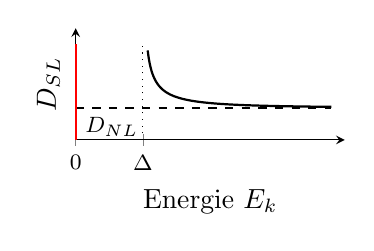
\begin{tikzpicture}
%\useasboundingbox (-1.3,-1.2) rectangle (10.2,4.7);
%\draw (-1,-1) rectangle +(12,5);

    \begin{axis}[ xlabel={  Energie $E_k$ }, ylabel= { $D_{SL}$ }, 
         width=50mm, height=30mm, 
        %ymode=log, 
     %   ymode=log,
         xmin = 0,
        xmax = 4,
         ymin  = 0,
         ymax = 3.5,
         %xmax=5.5, ymin = 0, ymax=7.5,
         axis x line=bottom,
         axis y line=left,
         % xmax= 2e5, unbounded coords=jump, ymin=0, ymax = 4
        % label style={font=\tiny},
         tick label style={font=\footnotesize},
        xtick = {0,1 }, 
        xticklabels  = {$0$, $\Delta$},
        ytick= \empty  ,
        clip= false,
     %  legend pos= north west,
     %  legend style={draw=none, font=\footnotesize}
    ]


%     \addplot[no marks,   thin, gray, domain=0:1.2]{25.8128 /14}; 
     




\addplot[domain=1:3.8 , samples=200, thick, restrict y to domain=0:3]{x / sqrt(x^2 -1) };
\draw[dashed] (0,1) node[below right] {\footnotesize $D_{NL}$} -- (3.8,1);
\draw[red, thick] (0,0) -- (0,3);
\draw[dotted] (1,0) -- (1,3);

 %\node[right] at (0,2) {\tiny C};

% \node at (1,22) {\tiny Sn};
% \node at (1,43) {\tiny Hg};
% \node at (1,74) {\tiny Pb};



    \end{axis}
\end{tikzpicture}

%\end{document}